\documentclass[11pt]{scrartcl}

\usepackage[top=1.5cm]{geometry}
\usepackage{url}
\usepackage{float}
\usepackage{listings}
\usepackage{xcolor}
\usepackage{graphicx}

\setlength{\parindent}{0em}
\setlength{\parskip}{0.5em}

\newcommand{\youranswerhere}{[Your answer goes here \ldots]}
\renewcommand{\thesubsection}{\arabic{subsection}}

\lstdefinestyle{dmrsql}{
  language=SQL,
  basicstyle=\small\ttfamily,
  keywordstyle=\color{magenta!75!black},
  stringstyle=\color{green!50!black},
  showspaces=false,
  showstringspaces=false,
  commentstyle=\color{gray}}

\lstdefinestyle{dmrJava}{
  language=JAVA,
  basicstyle=\small\ttfamily,
  keywordstyle=\color{magenta!75!black},
  stringstyle=\color{green!50!black},
  showspaces=false,
  showstringspaces=false,
  commentstyle=\color{gray}}

\title{
  \textbf{\large Projektaufgabe 2 } \\
  Phase 2 – Legen der Basis (2.5 P) \\
  {\large Datenmanagement jenseits von Relationen}
}

\author{
  Gruppen Nummer (e.g. A1, B5, B3) \\
  \large Lastname1 Firstname1, StudentID1 \\
  \large Lastname2 Firstname2, StudentID2 
}

\begin{document}

\maketitle\thispagestyle{empty}

Dieses Reporting Template dient der Vorbereitung der Abgabe von Phase 2.

\subsection*{Alternativer Import für Ansatz 2 (0.5 Punkte)}

Zeigen Sie das create table Statement für $A$ oder $B$. 

\begin{lstlisting}[style=dmrsql]
  CREATE TABLE new_A (i INT PRIMARY KEY, row INT[])
\end{lstlisting}

Zeigen Sie, wie die Matrizen $A$ und $B$ des Toy Examples für Ansatz 2 in der DB aussehen.

\begin{figure}[H]
  \begin{minipage}[b]{.4\linewidth}
    \begin{center}
      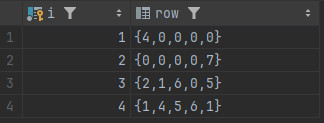
\includegraphics[width=\linewidth]{Tabelle_new_A.png}
      \caption{Tabelle A}
    \end{center}
  \end{minipage}
  \hspace{.1\linewidth}
  \begin{minipage}[b]{.4\linewidth}
    \begin{center}
      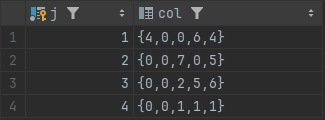
\includegraphics[width=\linewidth]{Tabelle_new_B.png}
      \caption{Tabelle B}
    \end{center}
  \end{minipage}
	\label{fig:}
\end{figure}

\subsection*{Ansatz 2 (0.5 Punkte):}

Geben Sie den Code der Funktion \texttt{dotproduct()} bzw. Ihrer Lösung für Ansatz 2 an.

\begin{lstlisting}[style=dmrsql]
public void ansatz2() {
  try (Statement statement = this.connection.createStatement()) {
    statement.execute("DROP TABLE IF EXISTS new_C");
    statement.execute("CREATE TABLE new_C ( " +
        + "i INT, j INT, val INT, PRIMARY KEY (i, j))");
    createFunction();
    statement.execute("INSERT INTO new_C (i, j, val) " +
      "SELECT new_A.i, new_B.j, dotproduct(new_A.row, new_B.col) " +
        "FROM new_A, new_B " +
        "WHERE dotproduct(new_A.row, new_B.col) != 0");
    } catch (SQLException e) {
        throw new RuntimeException(e);
    }
}

public void createFunction() {
  try (Statement statement = this.connection.createStatement()) {
    statement.execute("DROP FUNCTION IF EXISTS dotproduct(int[], int[])");
    statement.execute("CREATE OR REPLACE FUNCTION " +
        "dotproduct(vector1 int[], vector2 int[]) RETURNS int AS $$\n" +
        "DECLARE\n" +
        "    result int := 0;\n" +
        "BEGIN\n" +
        "    FOR i IN 1..array_length(vector1, 1) LOOP\n" +
        "        result := result + vector1[i] * vector2[i];\n" +
        "    END LOOP;\n" +
        "    RETURN result;\n" +
        "END;\n" +
        "$$ LANGUAGE plpgsql;");
    } catch (SQLException e) {
        throw new RuntimeException(e);
    }
}
\end{lstlisting}

Zeigen Sie für das Toy Example, dass $C$ korrekt berechnet wird (z.B. via Screenshot).

Wird korrekt berechnet, da die Ergebnisse übereinstimmen. Siehe Screenshots.
\begin{figure}[H]
  \begin{minipage}[b]{.4\linewidth}
    \begin{center}
      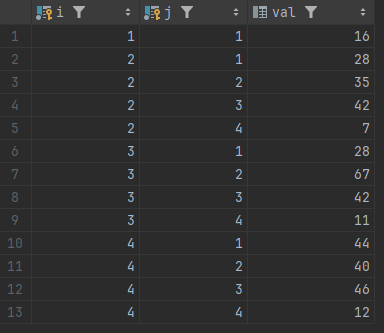
\includegraphics[width=\linewidth]{Tabelle_new_c.png}
      \caption{Tabelle C aus Arrays}
    \end{center}
  \end{minipage}
  \hspace{.1\linewidth}
  \begin{minipage}[b]{.4\linewidth}
    \begin{center}
      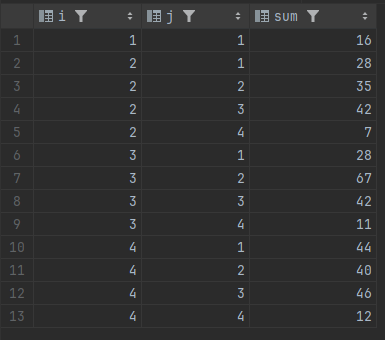
\includegraphics[width=\linewidth]{View_C_im_Vergleich.png}
      \caption{View C zum Vergleich}
    \end{center}
  \end{minipage}
	\label{fig:}
\end{figure}

\subsection*{Benchmark Definition (0.5 P):}

\begin{table}[h]
	\centering
		\begin{center}
			\begin{tabular}{ c c c }
				Parameter & Interval & Kommentar\\
				L & 2$^{3 + (n + 1)}$ & n $\leq$ 12 \\ 
				S & $((n + 1) \times 0.1)$ & n $\leq$ 8 \\  
			\end{tabular}
			\end{center}
	\caption{Getestet Matrixgrößen L und sparsity Werte S}
	\label{tab:MatrixgrößenLUndSparsityWerteS}
\end{table}

\youranswerhere{}

\subsubsection*{Auswertung (0.5 P)}

Stellen Sie Ihre Messergebnisse grafisch dar. 

\begin{figure}
	\centering

	\caption{Fügen Sie Ihre Resultate als Grafik ein}
	\label{fig:results}
\end{figure}


\subsection*{Zeitmamagement}

Benötigte Zeit pro Person (nur Phase 1): \textbf{5h}

\subsection*{References}

\begin{table}[H]
  \centering
  \begin{tabular}{c}
    \hline
    \textbf{Important:} Reference your information sources! \tabularnewline
    Remove this section if you use footnotes to reference your information sources. \tabularnewline
    \hline
  \end{tabular}
\end{table}

\end{document}
